\documentclass[11pt,a4paper]{article}
\usepackage[utf8]{inputenc}
\usepackage[T1]{fontenc}
\usepackage{amsmath,amssymb,amsfonts}
\usepackage{graphicx}
\usepackage[hidelinks]{hyperref}
\usepackage{booktabs}
\usepackage{natbib}
\usepackage{geometry}
\usepackage{tikz}
\usepackage{pgfplots}
\setlength{\emergencystretch}{2em}
\pgfplotsset{compat=1.18}
\usepackage{siunitx}
\sisetup{
  detect-all,
  input-symbols = (),
  table-number-alignment = center,
  group-digits = false
}
\usetikzlibrary{arrows.meta}
\geometry{margin=1in}

\title{Cognitive Amplification vs Cognitive Delegation in Human-AI Systems: A Metric Framework}
\author{Eduardo Di Santi \\
        University of Colorado Boulder}
\date{March 2026}

\begin{document}

\maketitle

\begin{abstract}
Artificial intelligence is increasingly embedded in human decision-making processes. In some cases, it enhances human reasoning; in others, it fosters excessive cognitive dependence. This paper introduces a conceptual and mathematical framework to distinguish \emph{cognitive amplification}---where AI improves hybrid human-AI performance while preserving and potentially strengthening human expertise---from \emph{cognitive delegation}, where reasoning is progressively outsourced to the AI system, risking long-term atrophy of human capabilities.

To characterize these regimes, we define four operational metrics: the Cognitive Amplification Index (CAI$^*$), which quantifies genuine collaborative gain beyond the best standalone agent; the Dependency Ratio ($D$) and Human Reliance Index (HRI), which measure the structural dominance of the AI within the hybrid output; and the Human Cognitive Drift Rate (HCDR), which captures the temporal erosion (or maintenance) of autonomous human cognitive performance under periodic evaluation. Together, these quantities define a low-dimensional metric space for classifying human--AI systems according to both immediate hybrid performance and long-term cognitive sustainability.

We validate the framework through an agent-based simulation in NetLogo across three reliance regimes and multiple dependency--atrophy configurations. The results distinguish degenerate AI-dominated delegation, human-preserving but weakly competitive interaction, and intermediate boundary regimes that approach the AI baseline while remaining structurally dependent. Across all tested configurations, no regime achieves genuine amplification: mixed reliance preserves substantially more human capability than full delegation, but still exhibits $CAI^* < 0$ and $D > 1$.

We further formulate a constrained optimization experiment over the atrophy parameter under the most favorable tested configuration. Reducing atrophy monotonically improves retained human capability, collaborative gain, and dependency structure, but even zero atrophy does not yield positive collaborative gain. This suggests that capability preservation alone is insufficient to recover genuine amplification under the present interaction dynamics.

The framework therefore provides a practical tool for evaluating not only whether human--AI systems perform well, but whether they do so in a way that preserves human capability over time. More broadly, it offers a basis for moving beyond simplistic accuracy metrics toward the analysis and design of systems that augment rather than silently displace human cognition.
\end{abstract}

\section{Introduction}

Artificial intelligence systems are no longer mere tools; they have become active participants in human cognitive processes. From diagnostic support in medicine to code generation in software engineering and literature synthesis in research, AI increasingly shapes how humans think, decide, and create. While this integration often yields impressive short-term performance gains, it also raises a fundamental question: does the AI truly \emph{amplify} human cognition, or does it gradually \emph{delegate} core reasoning tasks away from the human, leading to long-term dependence and skill erosion?

The distinction between cognitive amplification and cognitive delegation is not merely semantic. Amplification occurs when the human--AI team achieves results superior to what either could accomplish alone, while the human's independent capabilities remain intact or even improve over time. Delegation, by contrast, involves outsourcing significant portions of the cognitive workload to the AI, often resulting in hybrid outputs where the artificial component dominates and the human's unaided performance degrades with prolonged use.

Existing literature on automation bias, cognitive offloading, and extended cognition has documented these risks, yet few frameworks provide operational metrics to quantify and distinguish the two regimes in practice. Most evaluations still rely on aggregate accuracy or user satisfaction, metrics that fail to capture whether observed performance gains come at the cost of human cognitive sustainability. As a result, systems that appear effective in the short term may still conceal progressive dependence, loss of retained expertise, or only superficial forms of collaboration.

In this paper, we address this gap by proposing a compact mathematical framework built around four key quantities. The Cognitive Amplification Index (CAI$^*$) measures collaborative gain relative to the best standalone agent. The Dependency Ratio ($D$) and Human Reliance Index (HRI) quantify the structural balance of contribution within hybrid outputs. Most critically, the Human Cognitive Drift Rate (HCDR) tracks changes in autonomous human performance over time through periodic evaluation when AI assistance is temporarily withheld. Taken together, these metrics populate a low-dimensional phase space that makes visible the tension between short-term hybrid performance and long-term cognitive sustainability.

We argue that effective human--AI system design must satisfy a \emph{cognitive sustainability constraint}: hybrid performance $Q_{HA}$ should not be improved at the cost of degrading retained human capability over time. In formal terms, one should seek to maximize $Q_{HA}$ subject to $\text{HCDR} \geq 0$. Violating this principle leads to an ``automation trap'' --- a regime of apparently strong hybrid performance that conceals progressive deskilling or structural dependence on the artificial component.

To test the framework, we implement an agent-based simulation in NetLogo and evaluate three reliance regimes across multiple dependency--atrophy configurations. The results show that the proposed metrics distinguish degenerate delegation, human-preserving but weakly competitive interaction, and intermediate boundary regimes that approach the AI baseline while remaining structurally dependent. Across the tested configurations, no regime achieves genuine amplification, and a constrained optimization over the atrophy parameter shows that even eliminating atrophy is not, by itself, sufficient to recover positive collaborative gain.

The remainder of the paper is organized as follows. Section 2 formally defines the proposed metrics and derives their relationships. Section 3 presents the phase diagram and characterizes the resulting regimes. Section 4 discusses concrete design implications for current and future AI systems. Section 5 illustrates the framework with simple examples. Section 6 presents the agent-based simulation and experimental setup. Section 7 reports the main results. The paper then discusses the broader implications of the findings, outlines directions for future work, and concludes.

\section{Related Work}

\subsection{Human--AI collaboration and complementarity}

Recent work on human--AI collaboration emphasizes that the effectiveness of hybrid systems depends not only on the raw capabilities of the AI, but also on the quality of interaction, task structure, and the extent to which human and artificial agents contribute complementary information or capabilities. Research on complementarity in human--AI decision-making argues that productive collaboration emerges when differences in access to information, representational strengths, or error patterns can be productively combined, rather than when one agent merely replicates the function of the other.

Related studies further show that superior hybrid performance should not be taken for granted: in many settings, human--AI combinations fail to outperform the best standalone agent. This makes the design of effective interaction protocols a central challenge rather than a secondary implementation detail. These findings motivate evaluation frameworks that go beyond raw hybrid accuracy. If performance gains are highly contingent on how the interaction is organized, then assessment must also examine \emph{how} those gains are achieved and whether they preserve an active human cognitive role.

\subsection{Overreliance, automation bias, and cognitive offloading}

A substantial body of work has documented that humans frequently over-rely on automated decision aids. Research on automation bias describes the tendency of users to assign excessive weight to automated recommendations, reduce independent verification, and inherit system errors---particularly in high-stakes or cognitively demanding tasks. More recent literature on AI overreliance extends these concerns to contemporary generative systems, showing that AI assistance can subtly alter judgment strategies, reduce scrutiny, and create a misleading appearance of robust human oversight.

These issues connect closely to the literature on cognitive offloading. Studies in this area demonstrate that external aids can boost immediate task performance while simultaneously reshaping how users remember, reason, and allocate mental effort. In the context of AI-assisted decision-making, this raises a critical possibility: a system may improve short-term hybrid performance while weakening the user's unaided capacity to perform comparable tasks. This temporal distinction---between immediate gains and long-term cognitive effects---lies at the core of the present paper.

\subsection{Human-centred AI and cognitively sustainable interaction}

Human-centred AI has increasingly been framed not only as a question of usability or explainability, but as a broader design commitment to preserving meaningful human agency, oversight, and participation. From this perspective, effective human--AI interaction requires more than accurate model outputs: it demands interfaces and workflows that calibrate trust, support critique, expose uncertainty, and maintain the human's ability to reason independently about the task.

Nevertheless, current evaluation practices in human--AI systems continue to prioritize immediate hybrid performance. Far less attention has been devoted to whether interaction designs preserve---or erode---human competence over time. The present work contributes to this gap by introducing a metric framework that explicitly distinguishes performance gains reflecting genuine \emph{cognitive amplification} from those that mask progressive \emph{cognitive delegation}.

\subsection{Conceptual foundations of human and artificial cognition}

The distinction proposed here also draws on longer-standing conceptual debates concerning the nature of human cognition and artificial computation. Searle's Chinese Room argument \cite{searle1980} remains a canonical challenge to the claim that formal symbol manipulation alone constitutes understanding. While the present paper does not seek to resolve debates in the philosophy of mind, it highlights a relevant asymmetry: human and artificial systems may produce similar outputs while relying on fundamentally different underlying processes.

Complementary philosophical work by Byrne on computation, self-knowledge, and the transparency of belief formation further underscores the risk that treating AI as a functional substitute for reasoning may alter the human subject's relationship to their own cognitive processes \cite{byrne-minds-machines,byrne-kim-2012,byrne2018}. In a different but related vein, Solms emphasizes the embodied, affective, and homeostatic grounding of human cognition and consciousness, suggesting that human intelligence cannot be reduced to abstract information processing \cite{solms2021,solms-friston-2019}.

Taken together, these perspectives reinforce why the preservation of human cognitive competence should be treated as a first-class concern in the design and evaluation of human--AI systems. The present paper does not claim that these philosophical positions directly entail the proposed metrics; rather, they supply the conceptual background for treating cognitive sustainability as central rather than peripheral.

\section{System Model}

Consider a hybrid human--AI system $S$ composed of a human agent $H$ and an artificial agent $A$. We represent this coupling symbolically as
\begin{equation}
S = H + A,
\end{equation}
where the ``$+$'' symbol is not intended as a literal additive decomposition of intelligence, but as a compact notation for a coupled system whose effective behavior emerges from the interaction between both components.

Human intelligence involves forms of understanding, judgment, and self-monitoring that cannot be fully captured by any single performance metric. Nevertheless, to evaluate whether an AI system amplifies or displaces human cognitive function, an operational measure of task-relevant capability is required. We therefore define the effective problem-solving capacity of the system as
\begin{equation}
Q(S) = Q(H,A),
\end{equation}
where $Q$ denotes a domain-specific, operational measure of cognitive performance (e.g., accuracy, solution quality, decision correctness, or other task-appropriate indicators). This is explicitly \emph{not} a measure of general intelligence.

The standalone performance of the human is denoted
\begin{equation}
Q_H = Q(H),
\end{equation}
while the standalone performance of the AI agent is
\begin{equation}
Q_A = Q(A).
\end{equation}
The hybrid performance is then
\begin{equation}
Q_{HA} = Q(S) = Q(H,A).
\end{equation}

The central question addressed in this paper is not whether AI can fully reproduce human intelligence, but whether AI systems enhance human cognitive agency or progressively replace its practical exercise.
In the present simulation, the standalone AI performance $Q_A$ is operationalized as a fixed reliability parameter rather than as a task-adaptive model output.

\section{Cognitive Amplification}

In the ideal case, the AI functions as a genuine cognitive amplifier. The hybrid system exhibits synergy: machine assistance extends human problem-solving capacity without suppressing the active exercise of human judgment and self-monitoring.

This synergistic effect can be expressed conceptually as
\begin{equation}
Q_{HA} = Q_H + Q_A + \alpha \, Q_H Q_A,
\end{equation}
where $\alpha > 0$ represents the strength of the productive interaction between human and AI. When $\alpha > 0$, the coupled system produces a positive interaction term beyond the sum of the isolated contributions.

This expression should be interpreted as an idealized model of human--AI synergy rather than a literal empirical law. In practice, performance measures are typically bounded and strongly task-dependent, and hybrid performance rarely scales in a strictly multiplicative fashion. For this reason, the framework developed in the following sections relies on relative performance metrics that compare the hybrid output against the relevant standalone baselines of $H$ and $A$ individually. These relative metrics allow us to quantify amplification without assuming any particular functional form for the interaction.

\section{Metrics for Human--AI Collaboration}

The system model defines three core performance quantities: $Q_H$, $Q_A$, and $Q_{HA}$. From these we derive four operational metrics that, when interpreted jointly, characterize the regime of human--AI interaction. No single metric is sufficient; the most informative assessment requires reading them together.

\subsection{Cognitive Amplification Index}

The Cognitive Amplification Index ($CAI^*$) quantifies the relative performance gain of the hybrid system over the best standalone agent:
\begin{equation}
CAI^* = \frac{Q_{HA} - \max(Q_H, Q_A)}{\max(Q_H, Q_A)}.
\end{equation}

\begin{table}[htbp]
\centering
\begin{tabular}{lc}
\toprule
$CAI^*$ & Interpretation \\
\midrule
$> 0$   & Genuine cognitive amplification over best standalone agent \\
$= 0$   & Hybrid matches best standalone agent (no net gain) \\
$< 0$   & Integration reduces overall performance \\
\bottomrule
\end{tabular}
\caption{Interpretation of the Cognitive Amplification Index $CAI^*$.}
\label{tab:cai}
\end{table}

A positive $CAI^*$ is a necessary but not sufficient condition for true cognitive amplification. Short-term synergistic gains can coexist with increasing AI dominance and long-term erosion of human competence. Additional metrics are therefore required.

\subsection{Dependency Ratio and Human Reliance Index}

The Dependency Ratio ($D$) measures the extent to which hybrid performance is anchored in the AI component:
\begin{equation}
D = \frac{Q_A}{Q_{HA}}.
\end{equation}

High values of $D$ (approaching 1) indicate strong AI dominance and limited human contribution, consistent with patterns of overreliance and automation bias.

The complementary Human Reliance Index is defined as
\begin{equation}
HRI = 1 - D = \frac{Q_{HA} - Q_A}{Q_{HA}}.
\end{equation}

In the present simulation, $Q_A$ is operationalized as a fixed baseline parameter representing AI reliability rather than a task-dependent measured performance. As a result, the Dependency Ratio should be interpreted as a comparative dominance indicator rather than as a strict mixture coefficient. In particular, values exceeding 1 may arise when observed hybrid performance falls below the nominal AI baseline, indicating ineffective integration rather than literal over-contribution of the AI component.

\begin{table}[htbp]
\centering
\begin{tabular}{ccc}
\toprule
Range of $D$ & Range of $HRI$ & Qualitative regime \\
\midrule
$< 0.5$  & $> 0.5$ & Human-dominant \\
$0.5$--$0.8$ & $0.2$--$0.5$ & Balanced collaboration \\
$> 0.8$  & $< 0.2$ & AI-dominated (risk of delegation) \\
\bottomrule
\end{tabular}
\caption{Operational regimes based on Dependency Ratio ($D$) and Human Reliance Index ($HRI$).}
\label{tab:dependency}
\end{table}

These threshold ranges are heuristic and primarily intended for interpretive guidance. In the present simulation, where $Q_A$ is treated as a fixed baseline, empirical values of $D$ should be read comparatively rather than as hard-bounded contribution shares.

\subsection{Human Cognitive Drift Rate}

While $CAI^*$, $D$, and $HRI$ describe the system state at a given moment, the Human Cognitive Drift Rate ($HCDR$) captures the temporal evolution of unaided human performance:
\begin{equation}
HCDR = \frac{Q_H(t_2) - Q_H(t_1)}{t_2 - t_1},
\end{equation}
where $Q_H(t)$ is the human's performance measured without AI assistance through periodic ``AI-off'' assessments.

\begin{itemize}
\item $HCDR \geq 0$ (amplification regime): unaided human performance is preserved or improves over time.
\item $HCDR < 0$ (delegation regime): unaided human performance deteriorates, consistent with cognitive offloading and deskilling effects.
\end{itemize}

$HCDR$ is the metric most directly linked to long-term cognitive sustainability.

\subsection{Regimes of Human--AI Collaboration}

The metrics above define a compact state space for human--AI systems. In particular, the pair $(D, CAI^*)$ provides a useful low-dimensional representation, where $CAI^*$ captures performance synergy and $D$ reflects the balance of contribution.

Figure~\ref{fig:phase_diagram} presents a conceptual phase diagram in this space. The horizontal axis represents the Dependency Ratio $D$ (increasing AI dominance), while the vertical axis shows the Cognitive Amplification Index $CAI^*$. The Human Cognitive Drift Rate ($HCDR$) acts as a third dimension that determines whether a given regime is cognitively sustainable in the long term.

\begin{figure}[htbp]
\centering
\resizebox{0.92\textwidth}{!}{%
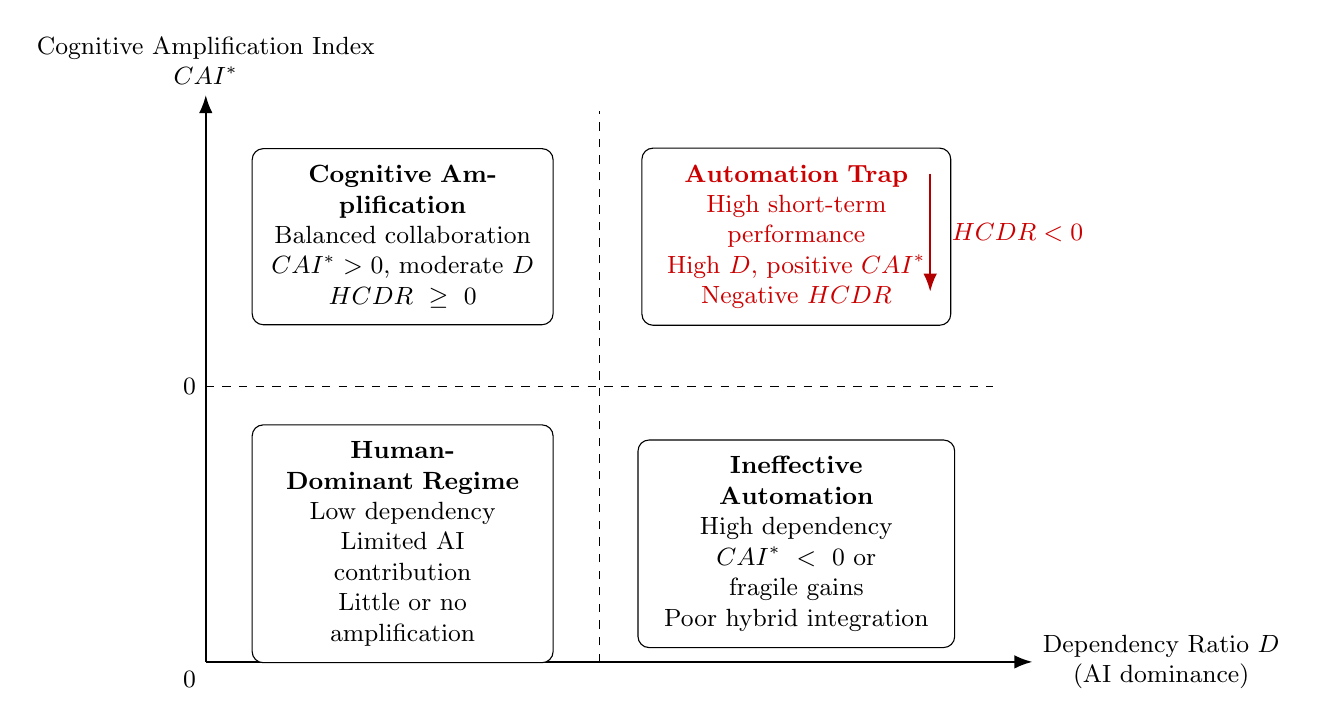
\begin{tikzpicture}[
    >=Latex,
    font=\small
]

\draw[->, thick] (0,0) -- (10.5,0)
    node[right, align=center] {Dependency Ratio $D$\\(AI dominance)};
\draw[->, thick] (0,0) -- (0,7.2)
    node[above, align=center] {Cognitive Amplification Index\\$CAI^*$};

\node[below left] at (0,0) {$0$};
\node[left] at (0,3.5) {$0$};

\draw[dashed] (5,0) -- (5,7);
\draw[dashed] (0,3.5) -- (10,3.5);

\node[
    align=center,
    text width=3.4cm,
    fill=white,
    draw,
    rounded corners,
    inner sep=6pt
] at (2.5,5.4)
{ \textbf{Cognitive Amplification}\\
Balanced collaboration\\
$CAI^* > 0$, moderate $D$\\
$HCDR \geq 0$ };

\node[
    align=center,
    text width=3.5cm,
    fill=white,
    draw,
    rounded corners,
    text=red!80!black,
    inner sep=6pt
] at (7.5,5.4)
{ \textbf{Automation Trap}\\
High short-term performance\\
High $D$, positive $CAI^*$\\
Negative $HCDR$ };

\node[
    align=center,
    text width=3.4cm,
    fill=white,
    draw,
    rounded corners,
    inner sep=6pt
] at (2.5,1.5)
{ \textbf{Human-Dominant Regime}\\
Low dependency\\
Limited AI contribution\\
Little or no amplification };

\node[
    align=center,
    text width=3.6cm,
    fill=white,
    draw,
    rounded corners,
    inner sep=6pt
] at (7.5,1.5)
{ \textbf{Ineffective Automation}\\
High dependency\\
$CAI^* < 0$ or fragile gains\\
Poor hybrid integration };

\draw[->, thick, red!70!black] (9.2,6.2) -- (9.2,4.7);
\node[right, text=red!80!black, align=left] at (9.35,5.45) {$HCDR < 0$};

\end{tikzpicture}%
}
\caption[Conceptual phase diagram of human--AI collaboration regimes]{Conceptual phase diagram of human--AI collaboration regimes. The horizontal axis represents the Dependency Ratio $D$, and the vertical axis represents the Cognitive Amplification Index $CAI^*$. The upper-right region corresponds to the \emph{automation trap}, where strong short-term hybrid performance coexists with high AI dominance and negative human cognitive drift.}
\label{fig:phase_diagram}
\end{figure}

These regimes demonstrate that maximizing short-term hybrid performance $Q_{HA}$ does not automatically guarantee cognitively sustainable collaboration. A system may exhibit positive $CAI^*$ and appear efficient while still operating in the automation trap if $HCDR < 0$. Conversely, a more balanced regime with moderate $CAI^*$ but non-negative $HCDR$ may be preferable when long-term human expertise is a priority.

\section{Design Implications}

The metric framework introduced above has immediate implications for the design and evaluation of human--AI systems. In safety-critical and knowledge-intensive domains, the objective should extend beyond maximizing short-term hybrid performance. The more demanding target is to support collaboration that preserves human capability over time, limits structural dependence on the artificial component, and, ideally, produces genuine collaborative gain.

From this perspective, three design goals become especially important:
\begin{itemize}
\item preserving or improving autonomous human performance over time ($HCDR \ge 0$),
\item avoiding regimes of excessive AI dominance, reflected in persistently high $D$ and low HRI,
\item and creating conditions under which the hybrid system can exceed the best standalone baseline ($CAI^* > 0$).
\end{itemize}

The present results do not, by themselves, validate specific interface prescriptions. However, the framework suggests several plausible design directions for moving systems away from delegation and toward amplification.

First, interaction protocols should keep the human actively inside the reasoning loop rather than positioning the AI as a final-answer oracle. Mechanisms such as mandatory human-first attempts, explicit hypothesis generation, or explanation-before-revelation may help reduce passive acceptance and preserve retained capability over time.\cite{cognitive-offloading,designing-ai-expertise,ai-pitfalls}

Second, AI systems should expose uncertainty, alternatives, and supporting evidence rather than presenting a single authoritative output for acceptance. This may help prevent structural overreliance and maintain a visible human contribution to the hybrid result.\cite{human-ai-uq,uncertainty-explainability,ai-cognitive-implications}

Third, cognitively sustainable deployment likely requires explicit capability-preservation mechanisms, including periodic AI-off evaluation, autonomous practice blocks, or training-oriented assistance modes. The optimization experiment reported in this paper suggests that preserving capability matters, but also that capability preservation alone is not sufficient to recover genuine amplification under the present interaction dynamics.

From an engineering standpoint, these implications suggest that human--AI systems should incorporate telemetry not only for output quality, but also for collaborative gain, dependency structure, and human cognitive drift. Such instrumentation would make it possible to detect when a system is moving from acceptable assistance toward hidden delegation, and would provide a basis for iterative redesign of both workflows and interaction policies.\cite{designing-intelligent-organization,automation-bias-ai-act}

\section{\texorpdfstring{Illustrative Measurement of $Q$}{Illustrative Measurement of Q}}

The framework introduced in this paper does not require a universal measure of intelligence. Instead, $Q$ denotes the effective problem-solving capability of a system within a specific task domain. In practice, $Q$ may be approximated using task-level performance measures such as decision accuracy, solution quality, task completion time, or error rates in controlled evaluation settings.

To illustrate the framework, consider a simplified engineering diagnostic task in which an operator must identify the root cause of a system anomaly from sensor signals. Suppose the following performance levels are observed:

\begin{center}
\begin{tabular}{lc}
\toprule
System & Diagnostic Accuracy \\
\midrule
Human alone ($Q_H$) & 0.70 \\
AI alone ($Q_A$) & 0.80 \\
Human + AI ($Q_{HA}$) & 0.92 \\
\bottomrule
\end{tabular}
\end{center}

The Cognitive Amplification Index is then

\begin{equation}
CAI^* = \frac{Q_{HA} - \max(Q_H, Q_A)}{\max(Q_H, Q_A)}
      = \frac{0.92 - 0.80}{0.80}
      \approx 0.15.
\end{equation}

The Dependency Ratio becomes

\begin{equation}
D = \frac{Q_A}{Q_{HA}} = \frac{0.80}{0.92} \approx 0.87,
\end{equation}

and the complementary Human Reliance Index is therefore

\begin{equation}
HRI = 1 - D \approx 0.13.
\end{equation}

In this example, the hybrid system clearly outperforms the best standalone component ($CAI^* > 0$), but the relatively high value of $D$ indicates that performance remains strongly anchored to the AI baseline. This illustrates an important point of the framework: positive collaborative gain does not by itself guarantee a balanced or cognitively sustainable regime. The same logic applies across domains such as medical decision support, industrial diagnosis, software engineering, or safety monitoring, provided that $Q$ is instantiated through an appropriate task-specific performance measure.

\section{Agent-Based Simulation for Empirical Validation}

To explore the dynamic consequences of cognitive amplification and cognitive delegation without exposing human participants to potentially harmful deskilling conditions, we implement an agent-based simulation in NetLogo. Agent-based modeling is well suited to this problem because it allows macro-level patterns of dependence, collaborative gain, cognitive drift, and adaptation failure to emerge from simple micro-level behavioral rules defined at the level of individual agents. NetLogo further provides a practical environment for large-scale stochastic experimentation, including systematic execution through BehaviorSpace.

\subsection{Purpose of the simulation}

The purpose of the simulation is not to reproduce human cognition in a psychologically complete sense, but to test whether the metric framework introduced in this paper can recover qualitatively distinct regimes of human--AI interaction under controlled assumptions. In particular, the simulation is designed to examine whether strong short-term hybrid performance can coexist with negative human cognitive drift, thereby producing the automation trap identified in the conceptual phase diagram.

The simulation therefore operationalizes the distinction between \emph{cognitive amplification} and \emph{cognitive delegation} in a stylized environment where agents face a stream of randomly generated tasks, decide whether to rely on an AI oracle, and update their internal skill state over time. The main observable of interest is whether repeated low-effort delegation improves immediate productivity while degrading the agent's autonomous capability when AI support is intermittently removed.

A further objective is to distinguish between competence that is merely preserved within a familiar task distribution and competence that remains robust under novelty. In many practical settings, the key risk of excessive delegation is not an immediate collapse in routine performance, but a progressive loss of adaptability when task structure changes. For this reason, the simulation also evaluates whether agents retain the ability to cope with previously unseen task configurations or shifts in the distribution of problem types after extended AI reliance.

\subsection{Agents, tasks, and skills}

Each agent represents a generic problem-solver rather than a novice learner. Agents are initialized with a non-zero baseline competence, reflecting the assumption that real operators typically begin with an already acquired set of task-relevant abilities. Formally, each agent $i$ is associated with a skill vector
\[
\mathbf{S}_i(t) = \left[s_{i1}(t), s_{i2}(t), \dots, s_{ik}(t)\right], \qquad s_{ij}(t) \in [0,1],
\]
where each component represents proficiency in one abstract cognitive skill dimension.

The initial condition is chosen such that agents already master part of the task space at the start of the simulation. This prevents trivial dependence on AI for tasks that are already familiar and forces the relevant dynamic to arise from exploration into less familiar regions of the problem space rather than from simple repetition of known routines.

Each task is represented as a requirement vector
\[
\mathbf{R}(t) = \left[r_1(t), r_2(t), \dots, r_k(t)\right], \qquad r_j(t) \in [0,1],
\]
together with a scalar difficulty parameter
\[
C(t) \in [0,1].
\]
Tasks are sampled randomly at each time step from a distribution over problem types and difficulty levels. In practice, the simulator uses a small set of abstract task families---analytical, diagnostic, sequential, and mixed---where each family activates a different subset of skill dimensions. This family-based representation preserves codable structure while allowing controlled shifts in the task distribution, thereby distinguishing performance on familiar tasks from performance under novelty or partial domain transfer.

\subsection{Task--skill mismatch, effort, and perturbation}

For each agent and task, the simulation computes a task--skill mismatch that approximates how demanding the task is relative to the agent's current internal capabilities:
\[
M_i(t) = \frac{1}{k} \sum_{j=1}^{k} \max\{0,\, r_j(t) - s_{ij}(t)\}.
\]
This quantity is low when the task lies within the agent's already mastered region and increases when the task requires capabilities that the agent has not yet sufficiently developed.

In addition to nominal task difficulty, the model includes a stochastic perturbation term representing unforeseen complications, contextual irregularities, or minor deviations from routine execution:
\[
\widetilde{C}(t) = C(t) + \epsilon(t),
\]
where $C(t) \in [0,1]$ is nominal difficulty and $\epsilon(t)$ is a bounded random perturbation. The perceived cognitive effort required to engage the task autonomously is then modeled as
\[
E_i(t) = \lambda_M M_i(t) + \lambda_C \widetilde{C}(t),
\]
with $\lambda_M, \lambda_C > 0$ as tunable parameters.

This construction is important for interpretation. The central issue is not whether agents can repeatedly solve already mastered tasks, but whether they continue to invest effort in cognitively demanding tasks that would expand or preserve competence. The effort term therefore acts as the main pressure driving agents toward either exploration or delegation, while the perturbation term ensures that routine competence is never evaluated under unrealistically frictionless conditions.

\subsection{Learning dynamics and cognitive atrophy}

The simulation is intentionally designed so that agents do not explicitly ``solve'' tasks in a symbolic sense. Instead, tasks act as opportunities for skill acquisition or skill erosion depending on the mode of interaction.

When the agent engages the task without AI support, the relevant skill dimensions are updated strongly. Let $\mathcal{A}(t)$ denote the subset of activated skill dimensions for the current task. Then the autonomous learning update is
\[
s_{ij}(t+1) = s_{ij}(t) + \alpha_{\mathrm{self}} \, (1 - s_{ij}(t)) \, r_j(t),
\qquad j \in \mathcal{A}(t),
\]
where $\alpha_{\mathrm{self}}$ is the self-learning rate. The factor $(1 - s_{ij}(t))$ induces diminishing returns near saturation and prevents unrealistic linear growth.

When the agent uses AI assistance, the same task produces only weak learning:
\[
s_{ij}(t+1) = s_{ij}(t) + \alpha_{\mathrm{AI}} \, (1 - s_{ij}(t)) \, r_j(t),
\qquad j \in \mathcal{A}(t),
\]
with
\[
0 < \alpha_{\mathrm{AI}} \ll \alpha_{\mathrm{self}}.
\]
Thus, AI use is not modeled as yielding zero learning, but as producing shallow acquisition relative to autonomous engagement.

To capture disuse effects, repeated AI reliance may also induce a downward drift in capability through an atrophy term with rate $\delta > 0$. In the present interpretation, atrophy is not merely a reduction in an abstract internal variable. Its practical significance is that it reduces autonomous robustness when task demands increase, when familiar tasks present unexpected complications, or when novel task structures are encountered. In this sense, cognitive atrophy represents a loss of resilience: agents may continue to function acceptably under routine conditions while becoming progressively less able to cope with perturbation, increased difficulty, or domain shift.

The central hypothesis is therefore that prolonged AI reliance may preserve acceptable local performance while weakening the deeper skill structure required for autonomous adaptation. In that case, the effect of delegation may remain partially hidden as long as the task environment stays familiar, and may become visible only when the agent is evaluated under altered or perturbed task conditions.

\subsection{Productivity, hybrid performance, and robustness}

Immediate task performance is modeled separately from long-term skill adaptation. If the agent uses the AI oracle, the task is completed with high short-term effectiveness, yielding strong instantaneous productivity. If the agent engages autonomously, immediate performance depends on its current skill profile, the mismatch of the task, and the effective difficulty of the current realization.

This separation allows the simulation to reproduce the central tension of the paper: a regime may exhibit strong short-term output while silently accumulating negative drift in autonomous capability.

At the population level, the simulation records mean autonomous skill level, AI usage frequency, immediate task productivity, estimated hybrid performance $Q_{HA}(t)$, autonomous performance $Q_H(t)$ measured during AI-off blocks, and autonomous performance under perturbed and novel task distributions. These observables allow direct estimation of the framework metrics introduced earlier, including $CAI^*$, $D$, and especially $HCDR$.

\subsection{AI-off evaluation and robustness probes}

To estimate Human Cognitive Drift Rate, the simulation periodically enters evaluation windows in which AI assistance is temporarily disabled. During these windows, autonomous performance is measured directly using the current skill vectors under the same task distribution used during normal interaction. Let $Q_H(t_m)$ denote the average autonomous performance measured at evaluation time $t_m$. The drift rate is approximated by
\[
HCDR \approx \frac{Q_H(t_{m+1}) - Q_H(t_m)}{\Delta t},
\]
where $\Delta t$ corresponds to the interval between evaluation windows.

A negative value indicates that repeated reliance on AI has degraded unaided capability over time, even if hybrid productivity remains high during normal operation. This AI-off protocol is critical because it distinguishes genuine cognitive amplification from operational dependence masked by strong AI performance.

In addition, the simulation includes two forms of robustness probe. \emph{Perturbation probes} introduce stochastic increases in difficulty for otherwise familiar task structures, producing a measure $Q_H^{\mathrm{pert}}(t)$. \emph{Novelty probes} sample tasks from shifted or reweighted task-family distributions, producing a measure $Q_H^{\mathrm{novel}}(t)$. These probes are executed periodically throughout the simulation rather than being restricted to a final evaluation stage. This allows the analysis to distinguish routine competence, robustness to variability within the same domain, and adaptive competence under distributional shift.

\subsection{Experimental phases}

The NetLogo simulation is organized into three phases.

\paragraph{Phase 1: Baseline without AI.}
Agents interact with randomly generated tasks using only autonomous learning. This establishes an initial trajectory of skill acquisition and provides a reference level for $Q_H$.

\paragraph{Phase 2: AI-assisted interaction.}
AI assistance becomes available, and agents interact with the AI oracle according to their assigned reliance regime. Periodic AI-off evaluation windows are introduced during this phase, enabling direct estimation of Human Cognitive Drift Rate ($HCDR$).

\paragraph{Phase 3: Shifted-environment stress test.}
In the final phase, the task distribution is modified to increase the prevalence of more complex or composite task families, effectively introducing a domain shift. AI assistance remains available, but the environment becomes less routine and more demanding in terms of generalization and transfer. Autonomous robustness is assessed through continued AI-off evaluation together with perturbation and novelty probes.

This three-phase structure makes it possible to distinguish baseline learning dynamics without AI, short-term hybrid performance under AI assistance, and longer-term robustness under distributional shift.

\subsection{Experimental protocol}

The experiments were implemented in NetLogo and executed through BehaviorSpace. We evaluated three reliance regimes as separate experimental modes: full delegation ($p_{\mathrm{AI}}=1.0$), minimal AI ($p_{\mathrm{AI}}=0.0$), and mixed reliance ($p_{\mathrm{AI}}=0.5$). These modes allow a clean comparison between maximal delegation, near-autonomous operation, and intermediate reliance under otherwise identical environmental conditions.

To probe different balances between capability erosion and dependency reinforcement, we studied three parameter configurations:
\begin{itemize}
\item \textbf{P0:} dependency-use-sensitivity $=0.2$, atrophy-delta $=0.004$
\item \textbf{P1:} dependency-use-sensitivity $=0.6$, atrophy-delta $=0.003$
\item \textbf{P2:} dependency-use-sensitivity $=0.4$, atrophy-delta $=0.002$
\end{itemize}

Unless otherwise stated, all remaining parameters were held fixed across experiments, including $N=1000$, $k=6$, $\alpha_{\mathrm{self}}=0.05$, and $\alpha_{\mathrm{AI}}=0.00105$. Each condition was repeated over 20 random seeds, and the reported metrics were aggregated over a final evaluation window rather than extracted from a single terminal step. For each run, we recorded the four principal quantities introduced in this paper---$CAI^*$, $D$, HRI, and HCDR---together with supporting observables such as autonomous performance, hybrid performance, retained skill, AI usage rate, and robustness under perturbation and novelty probes.

\section{Results}

We evaluated three experimental configurations, denoted P0, P1, and P2, each combining a different dependency-use sensitivity and atrophy rate. Within each configuration, we compared three reliance regimes: full delegation, minimal AI, and mixed reliance. All reported values are averaged over 20 random seeds.

Across all three configurations, the three reliance regimes separate clearly. Full delegation consistently collapses to a degenerate AI-dominated regime: AI usage saturates, retained human skill becomes minimal, and hybrid performance becomes indistinguishable from the AI baseline. Minimal AI preserves the highest autonomous human capability and the highest retained skill, but its hybrid performance remains substantially below the AI baseline, yielding strongly negative collaborative gain. Mixed reliance occupies an intermediate position in all configurations: it preserves substantially more human capability than full delegation and achieves hybrid performance much closer to the AI baseline than minimal AI, yet it still fails to produce genuine amplification, with $CAI^*<0$ and $D>1$ across seeds.

Under P2 (dependency-use-sensitivity $=0.4$, atrophy-delta $=0.002$), the mixed regime behaves as a boundary case. It retains moderate skill and autonomous performance while achieving hybrid performance close to the AI baseline. However, this apparent stability does not translate into positive collaborative gain: $CAI^*$ remains slightly negative and the dependency ratio remains above 1.

Under P1 (dependency-use-sensitivity $=0.6$, atrophy-delta $=0.003$), stronger dependency feedback pushes the mixed regime even closer to the AI baseline. In this setting, mixed reliance remains distinct from full delegation, but its hybrid behavior becomes more tightly coupled to AI performance, further suppressing the possibility of positive collaborative gain.

Under P0 (dependency-use-sensitivity $=0.2$, atrophy-delta $=0.004$), weaker dependency feedback reduces the aggressiveness of delegation, but higher atrophy still prevents amplification. In this configuration, mixed reliance uses AI less aggressively than in P1 or P2 and remains farther from the AI baseline, yet it still fails to achieve $CAI^*>0$.

Taken together, the experiments show that improved hybrid performance does not by itself imply cognitive amplification. Across all tested configurations, none of the reliance regimes achieves positive collaborative gain.

\begin{table}[htbp]
\centering
\small
\setlength{\tabcolsep}{4pt}
\begin{tabular}{
@{}
l
S[table-format=-1.4]
S[table-format=1.4]
S[table-format=1.4]
S[table-format=1.4]
S[table-format=-1.4]
S[table-format=1.4]
S[table-format=-1.4]
S[table-format=1.4]
@{}
}
\toprule
& \multicolumn{2}{c}{$CAI^*$}
& \multicolumn{2}{c}{$D$}
& \multicolumn{2}{c}{$HRI$}
& \multicolumn{2}{c}{$HCDR$} \\
\cmidrule(lr){2-3}
\cmidrule(lr){4-5}
\cmidrule(lr){6-7}
\cmidrule(lr){8-9}
Configuration (mixed regime) & {Mean} & {Std} & {Mean} & {Std} & {Mean} & {Std} & {Mean} & {Std} \\
\midrule
P0 $(0.2,\;0.004)$ & -0.0829 & 0.0039 & 1.0920 & 0.0050 & -0.0920 & 0.0050 & 0.0001 & 0.0037 \\
P1 $(0.6,\;0.003)$ & -0.0055 & 0.0012 & 1.0056 & 0.0012 & -0.0056 & 0.0012 & 0.0000 & 0.0037 \\
P2 $(0.4,\;0.002)$ & -0.0276 & 0.0031 & 1.0290 & 0.0030 & -0.0290 & 0.0030 & 0.0001 & 0.0037 \\
\bottomrule
\end{tabular}
\caption{Main framework metrics for the mixed-reliance regime across the three experimental configurations. Values are mean and standard deviation over 20 random seeds.}
\label{tab:mixed-configs}
\end{table}

\begin{table}[htbp]
\centering
\small
\setlength{\tabcolsep}{4pt}
\begin{tabular}{
@{}
l
S[table-format=-1.4]
S[table-format=1.4]
S[table-format=-1.4]
S[table-format=1.4]
S[table-format=-1.4]
S[table-format=1.4]
S[table-format=-1.4]
S[table-format=1.4]
@{}
}
\toprule
& \multicolumn{2}{c}{$CAI^*$}
& \multicolumn{2}{c}{$D$}
& \multicolumn{2}{c}{$HRI$}
& \multicolumn{2}{c}{$HCDR$} \\
\cmidrule(lr){2-3}
\cmidrule(lr){4-5}
\cmidrule(lr){6-7}
\cmidrule(lr){8-9}
Regime (P2) & {Mean} & {Std} & {Mean} & {Std} & {Mean} & {Std} & {Mean} & {Std} \\
\midrule
Full delegation & 0.0000 & 0.0000 & 1.0000 & 0.0000 & 0.0000 & 0.0000 & -0.0004 & 0.0039 \\
Minimal AI      & -0.2650 & 0.0190 & 1.4810 & 0.0420 & -0.4810 & 0.0420 & 0.0001 & 0.0038 \\
Mixed reliance  & -0.0276 & 0.0031 & 1.0290 & 0.0030 & -0.0290 & 0.0030 & 0.0001 & 0.0037 \\
\bottomrule
\end{tabular}
\caption{Framework metrics across reliance regimes under configuration P2. Values are mean and standard deviation over 20 random seeds.}
\label{tab:p2-regimes}
\end{table}

\subsection{Interpretation}

Taken together, the results provide an initial empirical validation of the proposed metric framework. The NetLogo simulation shows that the four quantities introduced in this paper are sufficient to distinguish several practically relevant human--AI regimes, including degenerate AI-dominated delegation, human-preserving but weakly competitive interaction, and intermediate boundary regimes that approach the AI baseline while remaining structurally dependent.

Most importantly, the experiments show that strong hybrid performance is not enough to establish genuine cognitive amplification. A regime may preserve more human capability than full delegation and still fail to achieve positive collaborative gain. In our simulations, the mixed-reliance regime repeatedly appears as such a boundary case: it can remain substantially more human-preserving than full delegation while still exhibiting $CAI^*<0$ and $D>1$.

This is precisely the distinction the framework is designed to detect. The results therefore support the main normative claim of the paper: evaluation of human--AI systems should not stop at observed hybrid performance, but must also account for dependency structure, retained human capability, and cognitive drift over time.

\subsection{Optimization experiment: reducing effective atrophy}

To test whether the proposed framework can support concrete design improvement, we performed a targeted optimization experiment over a single parameter: the atrophy rate $\delta$ (implemented as \texttt{atrophy-delta}). This parameter was selected because it has a direct intervention interpretation. In practical terms, lowering effective atrophy may correspond to measures such as mandatory autonomous practice, periodic AI-off assessment, scaffolded assistance, or training protocols designed to convert AI use into retained human capability rather than passive substitution.

The experiment was implemented directly in NetLogo BehaviorSpace. All simulation parameters were held fixed except $\delta$, which was varied over a predefined search range under the mixed-reliance regime. The purpose of the experiment was to determine whether controlling capability erosion alone is sufficient to move the system from a structurally dependent compromise regime toward genuine cognitive amplification. The constrained search procedure is described in Appendix~\ref{app:optimization}.

The search was conducted under configuration P2, which is the most favorable of the three baseline configurations for this one-parameter study, as it combines reduced atrophy with only moderate dependency reinforcement. If reducing atrophy alone were sufficient to recover genuine amplification, P2 is the most plausible tested setting in which such an effect would be expected to appear.

The evaluation criterion was defined in terms of the framework itself. In particular, we asked whether there exists a value of $\delta$ such that the resulting system satisfies positive collaborative gain ($CAI^* > 0$) while preserving human capability over time ($HCDR \ge 0$). This turns the optimization into a constrained search over the space of capability-preserving interventions.

Table~\ref{tab:atrophy-optimization} summarizes the outcome of the optimization experiment. The comparison is between the baseline mixed-reliance configuration and the best value of $\delta$ found by the search. The final column reports whether amplification, in the strict sense adopted in this paper, is attainable by acting on atrophy alone.

\begin{table}[ht]
\centering
\small
\setlength{\tabcolsep}{4pt}
\begin{tabular}{
@{}
l
S[table-format=1.4]
S[table-format=-1.4]
S[table-format=1.4]
S[table-format=1.4]
l
@{}
}
\toprule
Condition & {$\delta$} & {$CAI^*$} & {$D$} & {$HCDR$} & {Amplification} \\
\midrule
Baseline mixed & 0.0020 & -0.0276 & 1.0291 & 0.0001 & No \\
Best found     & 0.0000 & -0.0207 & 1.0218 & 0.0001 & No \\
\bottomrule
\end{tabular}
\caption{Best feasible result from the constrained search over $\delta$ under mixed reliance. Even at zero atrophy, reducing capability erosion alone does not produce genuine amplification.}
\label{tab:atrophy-optimization}
\end{table}

The full grid-search results for the atrophy-parameter optimization are reported in Appendix~\ref{app:atrophy-full-results}. These results confirm a monotonic improvement as $\delta$ is reduced, but also show that even the limiting case $\delta=0$ does not produce genuine amplification.

\begin{figure}[ht]
\centering
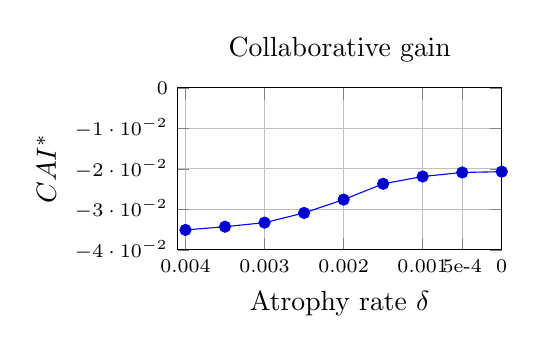
\begin{tikzpicture}
\begin{axis}[
    width=0.47\textwidth,
    height=0.30\textwidth,
    xlabel={Atrophy rate $\delta$},
    ylabel={$CAI^*$},
    xmin=0, xmax=0.0041,
    x dir=reverse,
    ymin=-0.040, ymax=0.000,
    xtick={0.004,0.003,0.002,0.001,0.0005,0},
    xticklabel style={font=\scriptsize},
    yticklabel style={font=\scriptsize},
    xticklabels={0.004,0.003,0.002,0.001,5e-4,0},
    ytick={-0.04,-0.03,-0.02,-0.01,0},
    scaled x ticks=false,
    scaled y ticks=false,
    grid=major,
    mark size=2pt,
    title={Collaborative gain}
]
\addplot+[mark=*] coordinates {
    (0.0040,-0.0351)
    (0.0035,-0.0343)
    (0.0030,-0.0333)
    (0.0025,-0.0309)
    (0.0020,-0.0276)
    (0.0015,-0.0237)
    (0.0010,-0.0219)
    (0.0005,-0.0209)
    (0.0000,-0.0207)
};
\addplot[dashed] coordinates {(0,0) (0.0041,0)};
\end{axis}
\end{tikzpicture}
\hfill
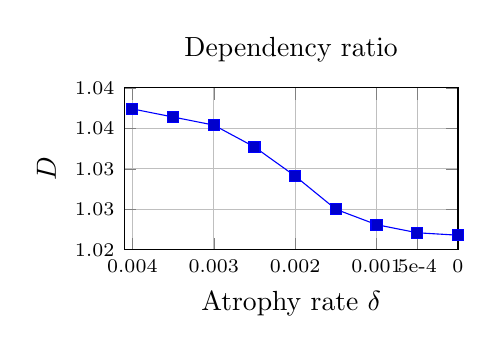
\begin{tikzpicture}
\begin{axis}[
    width=0.48\textwidth,
    height=0.30\textwidth,
    xlabel={Atrophy rate $\delta$},
    ylabel={$D$},
    xmin=0, xmax=0.0041,
    x dir=reverse,
    ymin=1.020, ymax=1.040,
    xtick={0.004,0.003,0.002,0.001,0.0005,0},
    xticklabel style={font=\scriptsize},
    yticklabel style={font=\scriptsize},
    xticklabels={0.004,0.003,0.002,0.001,5e-4,0},
    ytick={1.02,1.025,1.03,1.035,1.04},
    scaled x ticks=false,
    scaled y ticks=false,
    grid=major,
    mark size=2pt,
    title={Dependency ratio}
]
\addplot+[mark=square*] coordinates {
    (0.0040,1.0374)
    (0.0035,1.0364)
    (0.0030,1.0354)
    (0.0025,1.0327)
    (0.0020,1.0291)
    (0.0015,1.0250)
    (0.0010,1.0231)
    (0.0005,1.0221)
    (0.0000,1.0218)
};
\addplot[dashed] coordinates {(0,1.0) (0.0041,1.0)};
\end{axis}
\end{tikzpicture}
\caption{Effect of reducing the atrophy parameter \texorpdfstring{$\delta$}{delta} under mixed reliance. Moving from left to right corresponds to lower atrophy. Lower atrophy improves collaborative gain and reduces dependency, but even zero atrophy does not produce genuine amplification: \texorpdfstring{$CAI^*$}{CAI*} remains below zero and \texorpdfstring{$D$}{D} remains above 1 throughout the explored range.}
\label{fig:atrophy-optimization}
\end{figure}

This experiment isolates one practically meaningful design lever. Its purpose is not to solve the full human--AI design problem, but to determine whether capability-preserving intervention alone can be sufficient. The negative result indicates that genuine amplification requires coordinated control of multiple mechanisms rather than isolated mitigation of cognitive erosion.

\section{Discussion}

The framework proposed here does not attempt to measure intelligence in an absolute sense. Rather, it provides a relative metric system for evaluating whether human--AI interaction preserves, amplifies, or progressively displaces human cognitive capability.

The main contribution of the simulation is not merely to recover the familiar risk that strong short-term hybrid performance may coexist with long-term erosion of human capability. More importantly, it shows that a regime may remain apparently stable, preserve substantially more human capability than full delegation, and still fail to qualify as genuine amplification. In the experiments reported here, mixed reliance repeatedly occupies precisely this boundary position: it avoids outright collapse, approaches the AI baseline in hybrid performance, and yet remains structurally dependent, with negative collaborative gain and dependency above the balanced threshold.

This point matters because many practical evaluations of AI-assisted systems stop too early. A system that appears effective in terms of short-term output may still be structurally dependent on the artificial component, and may therefore fall short of true amplification even when the human agent has not yet visibly collapsed. The relevant distinction is therefore not simply between ``working'' and ``failing'' systems, but between systems that genuinely improve the joint cognitive unit and systems that merely maintain acceptable output under conditions of dependence.

This distinction is especially relevant in safety-critical and knowledge-intensive environments such as railway systems, aviation, pharmaceutical manufacturing, and medical technology. In such domains, the goal is not merely to achieve high nominal output, but to preserve robust human expertise under uncertainty, perturbation, and changing operational conditions. Excessive reliance on automation may therefore introduce a hidden form of fragility: systems can remain operationally efficient while progressively reducing the autonomy, adaptability, and resilience of the human component \cite{automation-bias,overreliance-ai}.

The experiments further suggest that cognitive delegation is not reducible to a single mechanism. It may arise through different combinations of dependency reinforcement and capability erosion. In some configurations, stronger dependency feedback pushes mixed reliance closer to effective delegation. In others, weaker behavioral feedback does not suffice to produce amplification when atrophy remains active. The optimization experiment strengthens this point: even under P2, the most favorable baseline configuration considered here, and even in the limiting case of zero atrophy, the system still fails to reach positive collaborative gain. This indicates that capability preservation matters, but is not by itself sufficient to recover genuine amplification under the present interaction dynamics.

From a design and evaluation standpoint, these results suggest a stronger claim than the original automation-trap formulation alone. Human--AI systems should not be judged solely by hybrid output, nor even by the absence of visible human collapse. They should instead be assessed through a joint lens that includes collaborative gain, dependency structure, retained human capability, and cognitive drift. Formally, the principle remains

\[
\max Q_{HA}
\quad \text{subject to} \quad
HCDR \ge 0,
\]

but the present results suggest that this condition is necessary rather than sufficient. A non-negative drift rate alone does not guarantee genuine amplification if the system remains structurally AI-dominated and fails to exceed the best standalone baseline. In other words, long-term preservation and collaborative gain must both be considered.

The broader implication is that genuine cognitive amplification may be substantially harder to obtain than conventional performance metrics suggest. This does not weaken the proposed framework; rather, it illustrates why such a framework is needed. Without metrics that jointly track collaborative gain, dependency, and retained human capability, one may easily mistake operational convenience for real augmentation.

The present work should therefore be understood not as a final theory of human--AI cognition, but as a decision-relevant evaluative lens. Its practical value lies in making visible whether a system is moving toward amplification, compromise, or delegation, and in showing that avoiding collapse is not the same as achieving genuine human--AI synergy.

\section{Future Work}

The present paper is primarily diagnostic rather than fully prescriptive. Its main contribution is to provide a compact metric framework for distinguishing among human-preserving, compromise, and delegation-dominated regimes of human--AI interaction. A central empirical lesson of the current study is that genuine amplification appears difficult to obtain even in comparatively favorable simulated conditions. Several natural extensions therefore follow from this foundation.

A first direction is technical and remains close to the scope of the current work. The proposed framework can be recast as the basis of a constrained optimization problem, in which a small number of design parameters---for example baseline AI reliance, dependency reinforcement, capability-preserving interventions, or interaction policies that affect learning under assistance---are adjusted so as to maximize collaborative gain while preserving human capability over time. In that setting, the relevant objective would not simply be to maximize hybrid output, but to search for regimes satisfying conditions such as $CAI^*>0$, $HCDR \ge 0$, and bounded dependency. This would allow the framework to move from regime identification toward principled search for viable amplification regions in parameter space.

A second direction concerns empirical grounding. The simulation developed here serves as a controlled stress test of the framework, but it remains an abstraction. Future work should therefore evaluate the proposed quantities in real human--AI interaction settings, particularly in domains where expertise retention, adaptation, and accountability are critical. Examples include industrial diagnosis, medical decision support, software engineering, and other environments in which AI assistance may improve immediate output while subtly altering long-term human competence.

A third direction concerns richer interaction design. In the present model, AI use is represented through stylized learning asymmetries, atrophy, and dependency feedback. Future work could examine more structured assistance policies, including delayed answer revelation, scaffolded hints, mandatory human-first attempts, periodic AI-off practice, or explanation-oriented assistance. Such mechanisms could be interpreted within the present framework as interventions that modify effective atrophy, dependency growth, or AI-mediated learning, thereby allowing systematic study of which design choices support genuine amplification rather than passive substitution.

Finally, broader normative and sociotechnical questions remain open. The framework introduced here can identify whether a system is moving toward amplification, compromise, or delegation, but it does not by itself determine what levels of autonomy, dependence, or expertise preservation ought to be considered acceptable in different institutional settings. Those questions extend beyond the present paper and may benefit from future work at the intersection of sociology, philosophy, human--computer interaction, education, and organizational studies. In that sense, the current work should be understood as an evaluative starting point: it offers a way to detect and compare cognitive regimes, while leaving the full normative and sociotechnical design problem for future research.

\section{Conclusion}

Artificial intelligence presents a dual possibility: it can strengthen human cognitive performance, or it can progressively displace the human role while preserving only the appearance of effective collaboration.

The metric framework proposed in this paper provides a way to analyze and monitor this distinction. Through a compact set of quantities---collaborative gain, dependency structure, human reliance, and cognitive drift---the framework makes visible differences that conventional performance evaluation can easily obscure. In particular, the agent-based experiments show that strong hybrid performance does not by itself imply genuine cognitive amplification. A regime may preserve more human capability than full delegation and still remain structurally dependent on the artificial component, failing to exceed the best standalone baseline.

The simulation results reported here distinguish three practically relevant regimes: degenerate AI-dominated delegation, human-preserving but weakly competitive interaction, and intermediate boundary regimes that approach the AI baseline while still failing to achieve positive collaborative gain. The optimization experiment strengthens this conclusion: even under the most favorable baseline configuration considered here, and even when atrophy is reduced to zero, genuine amplification is not recovered. This suggests that true human--AI amplification may be substantially harder to obtain than short-term performance measures alone would indicate.

The broader implication is that evaluating human--AI systems requires more than measuring immediate hybrid output. Systems should also be assessed in terms of whether they preserve human capability, avoid structural dependence, and support cognitively sustainable collaboration over time.

In safety-critical and knowledge-intensive domains, the goal of artificial intelligence should not be the silent replacement of human cognition, but the preservation and strengthening of expert judgment. Systems that increase automation while eroding retained human capability may ultimately reduce, rather than increase, the intelligence of the overall human--AI system.

Systems that improve output while degrading retained human capability may increase operational convenience, but they do not necessarily increase the intelligence of the overall human--AI system.

\section*{Code Availability}
The computational code supporting the findings of this study, including the NetLogo simulation and associated experimental materials required to reproduce the reported experiments, is publicly available at:
\url{https://github.com/eduardodisanti/cognitive_amplification_vs_delegation}

\bibliographystyle{plain}
\bibliography{references}

\appendix

\section{Optimization procedure}
\label{app:optimization}

To test whether capability-preserving intervention alone can produce genuine cognitive amplification, we performed a constrained parameter search over the atrophy rate $\delta$ (implemented as \texttt{atrophy-delta}) using NetLogo BehaviorSpace.

\subsection{Search space}

The search was restricted to the mixed-reliance regime, with all simulation parameters held fixed except $\delta$. We evaluated a predefined grid of candidate values:
    \[
\delta \in \{0.0040,\,0.0035,\,0.0030,\,0.0025,\,0.0020,\,0.0015,\,0.0010,\,0.0005,\,0.0000\}.
\]

Each candidate value was evaluated over 20 random seeds, using the same simulation horizon and final aggregation window as in the main experiments.

\subsection{Optimization criterion}

The search objective was defined in terms of the framework proposed in the main text. For each candidate value of $\delta$, we computed the mean values of $CAI^*$, $D$, and $HCDR$ across seeds. We then applied the following constrained selection rule:

\[
\delta^\star
=
\arg\max_{\delta}
\; CAI^*(\delta)
\quad
\text{subject to}
\quad
HCDR(\delta) \ge 0.
\]

Thus, the procedure seeks the value of $\delta$ that maximizes collaborative gain while excluding solutions that degrade human capability over time.

\subsection{Decision rule}

A candidate configuration was considered to achieve genuine amplification only if it satisfied both:
\[
CAI^* > 0
\qquad \text{and} \qquad
HCDR \ge 0.
\]

In the event that no candidate satisfies these conditions, the search still identifies the best attainable compromise under the imposed constraint. In that case, the optimization result is interpreted as evidence that reducing atrophy alone is insufficient to produce genuine amplification under the current interaction dynamics.

\subsection{Implementation}

The search was implemented directly in BehaviorSpace as a one-parameter sweep over \texttt{atrophy-delta}. For each value of $\delta$, the model was run over the full simulation horizon and the reported metrics were aggregated over the final evaluation window. This yields a reproducible and transparent constrained search procedure aligned with the metric framework introduced in the paper.

\subsection{Full results of the atrophy-parameter search}
\label{app:atrophy-full-results}
Table~\ref{tab:atrophy-grid-search} reports the full constrained search over the atrophy parameter $\delta$ under mixed reliance.
\begin{table}[htbp]
\centering
\resizebox{\textwidth}{!}{%
\begin{tabular}{
@{}
S[table-format=1.4]
S[table-format=-1.4]
S[table-format=1.4]
S[table-format=1.4]
S[table-format=1.4]
S[table-format=1.4]
S[table-format=1.4]
S[table-format=1.4]
S[table-format=1.4]
S[table-format=1.4]
S[table-format=1.4]
S[table-format=1.4]
S[table-format=1.4]
S[table-format=1.4]
S[table-format=1.4]
@{}
}
\toprule
& \multicolumn{2}{c}{$CAI^*$}
& \multicolumn{2}{c}{$D$}
& \multicolumn{2}{c}{$HCDR$}
& \multicolumn{2}{c}{$Q_H$}
& \multicolumn{2}{c}{Skill}
& \multicolumn{2}{c}{$Q_{HA}$}
& \multicolumn{2}{c}{AI use} \\
\cmidrule(lr){2-3}
\cmidrule(lr){4-5}
\cmidrule(lr){6-7}
\cmidrule(lr){8-9}
\cmidrule(lr){10-11}
\cmidrule(lr){12-13}
\cmidrule(lr){14-15}
{$\delta$}
& {Mean} & {Std}
& {Mean} & {Std}
& {Mean} & {Std}
& {Mean} & {Std}
& {Mean} & {Std}
& {Mean} & {Std}
& {Mean} & {Std} \\
\midrule
0.0040 & -0.0351 & 0.0032 & 1.0374 & 0.0034 & 0.0000 & 0.0037 & 0.6059 & 0.0269 & 0.3279 & 0.0086 & 0.9649 & 0.0032 & 0.8361 & 0.0153 \\
0.0035 & -0.0343 & 0.0031 & 1.0364 & 0.0033 & 0.0000 & 0.0037 & 0.6112 & 0.0270 & 0.3535 & 0.0096 & 0.9657 & 0.0031 & 0.8289 & 0.0157 \\
0.0030 & -0.0333 & 0.0029 & 1.0354 & 0.0031 & 0.0000 & 0.0037 & 0.6184 & 0.0265 & 0.3892 & 0.0115 & 0.9667 & 0.0029 & 0.8221 & 0.0166 \\
0.0025 & -0.0309 & 0.0028 & 1.0327 & 0.0029 & 0.0001 & 0.0037 & 0.6324 & 0.0266 & 0.4498 & 0.0131 & 0.9691 & 0.0028 & 0.8076 & 0.0184 \\
0.0020 & -0.0276 & 0.0031 & 1.0291 & 0.0033 & 0.0001 & 0.0037 & 0.6506 & 0.0267 & 0.5423 & 0.0142 & 0.9724 & 0.0031 & 0.7899 & 0.0182 \\
0.0015 & -0.0237 & 0.0032 & 1.0250 & 0.0034 & 0.0001 & 0.0037 & 0.6761 & 0.0254 & 0.6694 & 0.0117 & 0.9763 & 0.0032 & 0.7733 & 0.0189 \\
0.0010 & -0.0219 & 0.0033 & 1.0231 & 0.0034 & 0.0001 & 0.0037 & 0.6958 & 0.0249 & 0.7917 & 0.0068 & 0.9781 & 0.0033 & 0.7670 & 0.0192 \\
0.0005 & -0.0209 & 0.0033 & 1.0221 & 0.0035 & 0.0001 & 0.0037 & 0.7055 & 0.0236 & 0.8878 & 0.0039 & 0.9791 & 0.0033 & 0.7636 & 0.0194 \\
0.0000 & -0.0207 & 0.0032 & 1.0218 & 0.0034 & 0.0001 & 0.0037 & 0.7125 & 0.0227 & 1.0000 & 0.0000 & 0.9793 & 0.0032 & 0.7630 & 0.0194 \\
\bottomrule
\end{tabular}%
}
\caption{Constrained search over the atrophy parameter \texorpdfstring{$\delta$}{delta} under mixed reliance. Values are mean and standard deviation over 20 random seeds. Lower atrophy improves retained human capability and collaborative gain, but even zero atrophy does not yield positive collaborative gain.}
\label{tab:atrophy-grid-search}
\end{table}

\end{document}